\def\year{2019}\relax
%File: formatting-instruction.tex
\documentclass[letterpaper]{article} %DO NOT CHANGE THIS
\usepackage{aaai19}  %Required
\usepackage{times}  %Required
\usepackage{helvet}  %Required
\usepackage{courier}  %Required
\usepackage{url}  %Required
\usepackage{graphicx}  %Required
\frenchspacing  %Required
\setlength{\pdfpagewidth}{8.5in}  %Required
\setlength{\pdfpageheight}{11in}  %Required

\nocopyright
\usepackage[noend]{algpseudocode}
\usepackage{algorithm}


%PDF Info Is Required:
  \pdfinfo{
/Title (Comparing Some Bayesian Filtering Techniques)
/Author (Abheek Ghosh)}
\setcounter{secnumdepth}{0}  
 \begin{document}
% The file aaai.sty is the style file for AAAI Press 
% proceedings, working notes, and technical reports.
%
\title{Comparing Some Bayesian Filtering Techniques}
\author{Abheek Ghosh\\
Department of Computer Science \\
The University of Texas at Austin \\
2317 Speedway, Stop D9500 \\
Austin, TX 78712 \\
}
\maketitle
\begin{abstract}
We investigate and compare Bayesian filtering algorithms, methods like particle filter. The filtering algorithms we implement are: fixed size grid (histogram) filter, tree based dynamic grid (histogram) filter, particle filter, filter based on a polynomial of fixed degree, and a filter based on feed-forward deep neural networks. We develop a modular testing and simulation framework where these techniques and possibly other filtering techniques can be compared. Assuming that the estimation of a very very fine grid filter is the best that can be generated using the past history of samples, we compare the algorithms on the basis of: the error in the estimated mean state of the system, and the $L_2$-error in the cumulative distribution function of the estimated belief.

We observe that for the localization of Nao robot, particle filter works better than other techniques given same computation resources. We anticipate that this is due to combination of factors: the high error in the vision samples, simple belief distribution, non-requirement of high accuracy in state estimation. When we need very high accuracy and deterministic behavior, techniques like dynamic grid filter and neural network perform better.
\end{abstract}

\noindent

\section{Introduction}
Uncertainty is ubiquitous in robotics, which has made probabilistic algorithms an essential part of it. One of the most important uses of the probabilistic algorithms is for the estimation of the state of a robot. The general algorithm used for this is the Bayesian filtering algorithm, pseudocode given below:

\begin{algorithm}
\caption{Bayes-Filter}\label{bayes_algo}
\begin{algorithmic}[1]
\Require{$bel(x_{t-1})$, $u_t$, $z_t$}
\State{for all $x_t$ do}
\State{\quad $\overline{bel(x_t)}$ = motion\_update($bel(x_{t-1})$, $u_t$)}
\State{\quad $bel(x_t)$ = sensor\_update($\overline{bel(x_t)}$, $x_t$)}
\State{end for}
\State \textbf{return} $bel(x_t)$ 
\end{algorithmic}
\end{algorithm}

In the above algorithm, the time is discrete and denoted by $t$. $x_t$ is the random variable representing the state at time $t$. Similarly, $u_t$ is the motion measurement and $z_t$ is the sensor measurement at time $t$. $bel(x_t)$ denotes the belief distribution. The motion\_update updates the belief using the previous belief and current action measurement, and the sensor\_update, similarly, updates the belief using current sensor measurement.

To practically implement a fast and resonably accurate Bayesian filtering algorithm we need to decide upon these three main points:
\begin{enumerate}
\item Efficiently store/approximate the belief distribution $bel(x_t)$. The belief is essentially a probability distribution function. Some of the common methods used for function approximation are:
\begin{itemize}
	\item Storing the value of the function at a finite number of points in the domain.
	\item Using a finite degree polynomial that fits the function with least squared error.
	\item Recently very popular and successful in several other areas, using a deep neural network.
	\item As the belief is a PDF with its special properties, it is non-negative and sums (integrates) up to $1$, we can store it using fixed number of samples from the distribution.
\end{itemize}
\item Efficiently do the motion update. If the motion measurement has, or can be easily transformed into one that has, the same dimension as the state, and each dimension of the motion measurement has one-to-one correspondence to that of the current state, then usually the update in the belief looks similar to translation of the function.
\item Efficiently do the sensor update. This mainly involves finding the product of two PDFs.
\end{enumerate}

The ideas mentioned in the (1) above motivate the techniques we study. But, as we will see later, (2) and (3) will have a significant impact on the performance of the algorithms.

For our project, we assume that the state, the motion measurement, and the sensor measurement have the same number of dimensions with one-to-one correspondence among the dimensions. This helps simplify the algorithms and our testing and simulation framework. We also assume that motion and sensor measurements can be queried by the algorithm in constant time.
\section{Related Work}
For linear systems with white noise, Kalman filter (KF)~\cite{kalman,prob} is the optimal Bayesian filter algorithm and is used popularly. But KF doesn't work well for non-linear systems. For non-linear systems, the extended Kalman filter (EKF)~\cite{prob} is one of the most popular filtering algorithms. EKF is usually implemented using a first order Taylor expansion, but higher order EKFs have also been used. Although the EKF (in its many forms) is a widely used filtering strategy, over several decades of experience with it has led to a general consensus within the tracking and control community that it is difficult to implement, difficult to tune, and only reliable for systems which are almost linear on the time scale of the update intervals~\cite{ukf1}. We implemented KF and EKF for assignment 4 ball tracking.

Unscented Kalman filter (UKF) is an extension of KF and EKF. It was introduced by~\cite{ukf1,ukf3} with the accuracy of EKF with second-order Taylor approximation, and improved by~\cite{ukf2} to make its accuracy comparable to third order. In UKF, a set of appropriately chosen weighted points are used to parameterize the means and covariances of the probability distributions. UKF has the same time complexity as first-order EKF while mitigating the sub-optimal performance and possible divergence.

Another aimilar algorithm is the Gaussian sum filter introduced in~\cite{gpf}. In this method, there is a weighted sum of multiple non-correlated Gaussian particles. As a sum of Gaussian distributions is a Gaussian distribution, the estimated distribution is also Gaussian. In the paper, they show that under the Gaussianity assumption, the Gaussian particle filter is asymptotically optimal in the number of particles and, hence, has much-improved performance and versatility over other Gaussian filters, especially when nontrivial nonlinearities are present. On the other hand, it has lower complexity than particle filters.

The simplest non-parametric technique is the grid (histogram) algorithm. An extension to grid algorithm is the dynamic grid algorithm~\cite{grid1,prob}. In this algorithm, the grid is dynamically resized if the probability mass in the grid goes above a certain threshold. We implement these algorithms along with particle filter, they will be described in detail in the next section.

A different approach for filtering that we looked into is where the belief distribution is stored using a neural network. \cite{neuspike1} mention that organisms acting in uncertain dynamical environments often employ exact or approximate Bayesian statistical calculations in order to continuously estimate the environmental state, integrate information from multiple sensory modalities, form predictions and choose actions. They study how these computations could have been implemented in the neural network, and introduce the spike neural networks. Other relevant works used a recurrent neural network (RNN) to learn the internal behavior of the dynamic system, and a feedforward neural network attached to the RNN that outputs the estimated state~\cite{neu5,neu1,neu2}. Another paper~\cite{neu4} used a multilayer network that approximates the posterior, and gives output the state estimate when subjected to unknown noises.

Several analytical techniques are also used for filtering~\cite{anl1,anl2,anl3}. We mentioned only a few papers, but there is an enormous literature related to filtering, estimation theory, and their use in probabilistic robotics. 
\section{Algorithms and Implementation}
In this section, we describe the filtering algorithms we used: fixed size grid filter, tree-based dynamic grid filter, particle filter, filter based on a polynomial of fixed degree, and a filter based on feed-forward deep neural networks. We implemented the algorithms in C++, the simulation data was generated using Octave (Matlab). The source code is available at \textit{https://github.com/AbheekG/filter}. We used the Eigen library and some code from \textit{https://github.com/yixuan/MiniDNN/} to implement the feed-forward neural network. For running in Nao, the LARG codebase given to the class was used.

The \textit{Filter} C++ class contains the parameters and functions common to all filtering algorithms, like sensor and motion measurement functions, timing functions, I/O, etc. Each individual algorithm has its own derived class.

\subsection{Particle Filter}
It is similar to what we did in assignment 5 (localization), with slight modifications to fit our testing framework. The class \textit{ParticleFilter} implements this algorithm. The number of particles is given as the hyper-parameter.

\subsection{Fixed Grid Filter}\label{gf_def}
In this method, the entire state space is divided into a grid of a fixed number of points. For each grid point, the value of the belief distribution is stored. The grid structure is pre-decided and doesn't change with the time or the belief distribution.

The algorithm works for any arbitrary dimension and grid size. Each grid is a hyperrectangle, e.g., a rectangle for 2-D. It stores the function values in a linear vector with appropriate indexing for multi-dimension. The class \textit{GridFilter} implements this algorithm. The grid size is given as the hyper-parameter.

\begin{figure}
\caption{Fixed grid filter. (Figure taken from \cite{prob})}
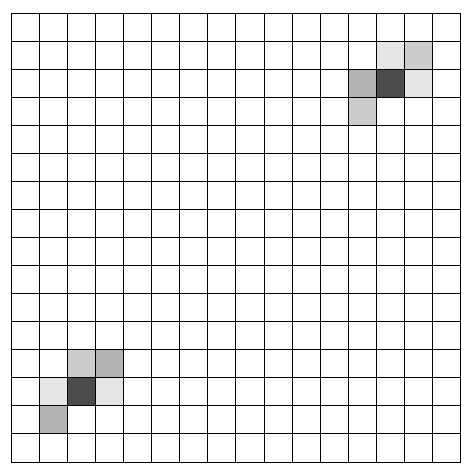
\includegraphics[width=\linewidth]{grid}
\end{figure}

\subsection{Dynamic Grid Filter}
Similar to the fixed grid filter\ref{gf_def}, in this method also the entire domain of the belief distribution is divided into sub-domains (grid block) and the value of the belief distribution is approximated for each grid block.

The entire grid is stored in the form of a tree. Each node corresponds to a grid block. A node of the tree is a leaf node if the total probability (weight) for the grid block (hyperrectangle) corresponding to the node is less than a given probability threshold. If the weight of a node is more than the probability threshold then its grid block is partitioned into its children. For example, the root of the tree has a grid block with the size of the entire domain for the robot state and probability $1$. If the probability threshold is less than $1$ then the root will have children.

The nodes are branched and collapsed dynamically as the belief distribution changes. A node whose weight goes above the threshold is branched, while if it goes below the threshold it is collapsed and its children vanish. We also have a partial implementation for using different lower and upper probability thresholds. The class \textit{DynamicGridFilter} implements this filtering method. The probability thresholds are given as the hyper-parameters.

\begin{figure}
\caption{Dynamic grid filter. (Figure taken from \cite{prob})}
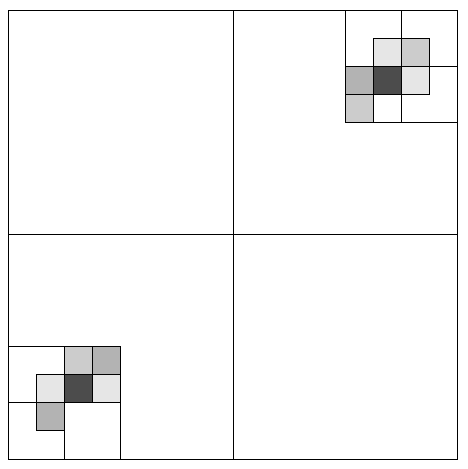
\includegraphics[width=\linewidth]{dgrid}
\end{figure}

\subsection{Polynomial Filter}
In this method, we approximate the belief using a polynomial of fixed degree. The original state is converted to a new modified state with higher order terms, and then the least square fit is done to find the coefficients of the polynomial. The class \textit{PolynomialFilter} implements this algorithm. The degree is given as a hyperparameter. Due to lack of time, we could only have implementation up to degree $2$.

\subsection{Neural Network Filter}
In this method, we use a feed-forward deep neural network (NN). The input to the neural network is a state and output is the value of the belief distribution corresponding to the state. Essentially, the function represented by the NN is the approximate belief distribution. The neural network is partially trained in each time step (sensor and motion update). For each time step, the input data (set of states), $X$, is generated depending on the previous belief (or NN), more samples from areas with higher weight and less from the lower weight. The output data, $y$, is generated as a product of current sensor measurement and previous belief. Currently, the motion is updated by doing a shift in the $X$, assuming that motion updates don't have an error.

The class \textit{NeuralNetwork} implements this algorithm. All the standard hyper-parameters for a neural network, like the number of layers, size of each layer, learning rate, batch size, etc. are applicable here also.
\section{Results}
We evaluated the algorithms on several tests (included with the code, in $data$ folder). Some of the generated tests were simpler, other more complex. We well present data for two of them. We also ported the fixed grid filter and dynamic grid filter algorithms on Nao robot and did the practical demonstration.

In the first test, we have only one dimension. Initially, there are three states around which the robot can be. With time the robot's confidence increases for one location. All the techniques have around $100$ parameters. (Except polynomial filter which has implementation upto only degree $2$, so $3$ parameters only.)
\begin{itemize}
	\item Particle filter (PF): $100$ particles.
	\item Fixed grid filter (FGF): $100$ grid points.
	\item Dynamic grid filter (DGF): $50$ to $100$ grid points. (dynamic.)
	\item Neural network (NN): Two layers of size $10$. $10*10=100$. (approx.)
\end{itemize}

\begin{table}
\caption{Error in mean of estimated state.}	
\begin{center}
\begin{tabular}{ | c || c | c | c | c | c | }
Step & PF & FGF & DGF & PolyF & NN \\
1 & 0.5007 & 0.0010 & 0.1915 & 0.0224 & 0.0259 \\  
2 & 0.6320 & 0.0015 & 0.4271 & 0.2390 & 0.2663 \\  
3 & 0.3487 & 0.0018 & 0.7181 & 0.3715 & 0.4382 \\  
4 & 0.1031 & 0.0020 & 1.0043 & 0.5999 & 0.4570 \\  
5 & 0.3854 & 0.0021 & 1.2934 & 0.5197 & 0.2080 \\  
6 & 0.4882 & 0.0022 & 1.4082 & 0.0116 & 0.0971 \\  
7 & 0.4264 & 0.0023 & 1.3687 & 0.8871 & 1.0026 \\  
8 & 0.1852 & 0.0023 & 1.2192 & 1.8244 & 1.5367 \\  
9 & 0.0173 & 0.0023 & 1.0895 & 2.7725 & 2.1200 \\  
10 & 0.2027 & 0.0023 & 0.9733 & 3.5915 & 2.3507 
\end{tabular}
\end{center}
\end{table}

\begin{table}
\caption{L2-error in computed CDF.}	
\begin{center}
\begin{tabular}{ | c || c | c | c | c | c | }
Step & PF & FGF & DGF & PolyF & NN \\
1 & 5.5895 & 0.3385 & 5.6089 & 4.7394 & 5.5770 \\  
2 & 3.1485 & 0.3799 & 4.7029 & 7.9123 & 8.0532 \\  
3 & 5.1527 & 0.4117 & 5.0591 & 8.9555 & 8.0353 \\  
4 & 4.5226 & 0.4256 & 5.4113 & 9.6027 & 7.7276 \\  
5 & 9.2158 & 0.4360 & 6.1948 & 10.0842 & 8.2515 \\  
6 & 7.7962 & 0.4820 & 5.6106 & 13.5393 & 9.0468 \\  
7 & 7.1645 & 0.5667 & 4.6130 & 18.8865 & 14.8883 \\  
8 & 7.4783 & 0.6547 & 4.0991 & 21.6299 & 12.3882 \\  
9 & 5.9185 & 0.7172 & 3.4860 & 22.7425 & 12.8611 \\  
10 & 5.7165 & 0.7603 & 3.0654 & 22.6650 & 10.1677 
\end{tabular}
\end{center}
\end{table}

\section{Conclusion}
In this project, we used some standard filtering techniques, like the grid filter (fixed and dynamic) and the particle filter, and some slightly unconventional ones, like the polynomial filter and the neural network. We made the algorithms work on both simulation and Nao, albeit they didn't perform very well. The algorithms were far more complex to implement than particle filter, but performed worse than particle filter. Some possible reasons that the algorithms didn't work well:
\begin{itemize}
	\item The sub-algorithms used for incorporating sensor and motion updates as part of the individual filtering algorithms may not be the best way to do it. For example, in the dynamic grid filtering algorithm, for sensor update of each grid block we have to reach the full depth of the tree multiple times. For some motion updates, the entire tree has to be reconstructed.
	\item The implementation of the algorithms is not efficient.
	\item In areas where the polynomial methods and neural networks are used and the neural networks have given tremendous results, the estimated function doesn't vary over time. The NNs have to learn a complex fixed function using a lot of samples. In our case, the belief distribution varies over time. In some experiments, we found that once the neural network is already trained it gets stuck there and cannot approximate an entirely new function.
	\item The belief distributions are not very complex, atleast for the examples we constructed and for Nao's localization.
	\item The error in sensor and motion measurements is very high. The high accuracy provided by deep NNs becomes irrelevant here.
\end{itemize}

\section{Acknowledgements}
We thank Prof. Peter Stone and TA Josiah Hannah for their guidance, regular valuable comments, and providing us with the Nao robot and appropriate development environment.


\bibliographystyle{aaai}

\bibliography{references}

\end{document}
